% ------------------------------------------------------------%
% 2015-2021 - Emerson Ribeiro de Mello <mello@ifsc.edu.br>
% ------------------------------------------------------------%
% Sets aspect ratio to 4:3, and frame size to 128 mm by 96 mm
\documentclass{beamer}
% Sets aspect ratio to 16:9, and frame size to 160 mm by 90 mm.
% \documentclass[aspectratio=169]{beamer}
% Sets aspect ratio to 16:10, and frame size to 160 mm by 100 mm.
% \documentclass[aspectratio=1610]{beamer}

% -------------------------------------------------%
%  Package options
% -------------------------------------------------%
% 
% textbgcolor   - frametitle background color. default: 0d4f4d
% textfgcolor   - frametitle foreground color. default: ffffff
% slidebgcolor  - slide background color. default: eef1ec
% slidefgcolor  - slide text foreground color. default: 000000
% authorfgcolor - author, institute and date color. default: 000000
% itemsep - space between items (itemize, enumerate). default: 7pt
\usepackage[textbgcolor=0d4f4d,textfgcolor=ffffff,itemsep=7pt]{../0-ifscyan-modelo/beamerthemeifscyan}
% -------------------------------------------------%

% A good place to get some colors
% https://material.io/resources/color/#!/?view.left=0&view.right=0&primary.color=0d4f4d
% cyan: #0D4F4D, light: #417b79,  dark: #002625
% IFSC green: normal: #32A041, light: #69d26f, dark: #007013
% IFSC red: normal: #C8191E, light: #ff5747, dark: #8f0000 
% Other colors for textbgcolor
% purple 4527a0, blue 0d47a1, grey 546e7a, redwine 880e4f, brown 6d4c41, yelllow (bg=#fbc02d, fg=000000)

% Logo
\pgfdeclareimage[height=.4\paperheight]{ifsclogo}{../0-ifscyan-modelo/figs/ifsclogo.pdf}


% -------------------------------------------------%
%              Título 
% -------------------------------------------------%
\title{Minha aula sobre \LaTeX~Beamer}
\subtitle{Aula 01}
\author{Prof. Emerson Ribeiro de Mello}
\institute{%
\href{mello@ifsc.edu.br}{mello@ifsc.edu.br}%
}%
\date{26/09/2019}
% -------------------------------------------------%

% -------------------------------------------------%
%  Início do documento 
% -------------------------------------------------%
\begin{document}

\begin{frame}[plain]
    \titlepage
\end{frame}

\begin{frame}[plain, noframenumbering]{Licenciamento}
    \licenciamentoLivre
\end{frame}

\begin{frame}[plain, noframenumbering]{Sumário}
    \tableofcontents
\end{frame}


\jsonp
\lstset{numbers=none}

\begin{frame}{Esse tema usa fonte Roboto}
\begin{alertblock}{Como instalar a fonte Roboto no Linux}
     \texttt{sudo apt install texlive-fonts-extras}
\end{alertblock}
\end{frame}

\begin{frame}[fragile]{Visual Studio Code como IDE \LaTeX~para slides com Beamer}
\begin{enumerate}
    \item Instale a extensão LaTeX Workshop
    \item Vá em preferências \(\rightarrow\) \textit{User Snippets} e abra o arquivo \texttt{latex.json}
    \item Adicione as linhas abaixo dentro do arquivo \texttt{latex.json} e salve
\end{enumerate}

\begin{lstlisting}
{
"Beamer frame":{
    "prefix": "frame",
    "body": ["\\begin{frame}{$1}\n\\begin{itemize}\n\t\\item $2\n\\end{itemize}\n\\end{frame}"],
    "description": "Frame para LaTeX Beamer"
},
    "LaTeX itemize env":{
    "prefix": "itemize",
    "body": ["\\begin{itemize}\n\t\\item $1\n\\end{itemize}"],
    "description": "itemize env para LaTeX"
}
}
\end{lstlisting}
\begin{itemize}
    \item Isso permitirá que quando estiver editando o \texttt{.tex},  basta digitar ``frame'' ou ``itemize'' e pressionar ENTER para ele gerar o bloco.
\end{itemize}
\end{frame}


\begin{frame}{Um slide simples}
\begin{itemize}
    \item Abaixo uma figura ilustrando vários ramos do git
\end{itemize}
\begin{center}
    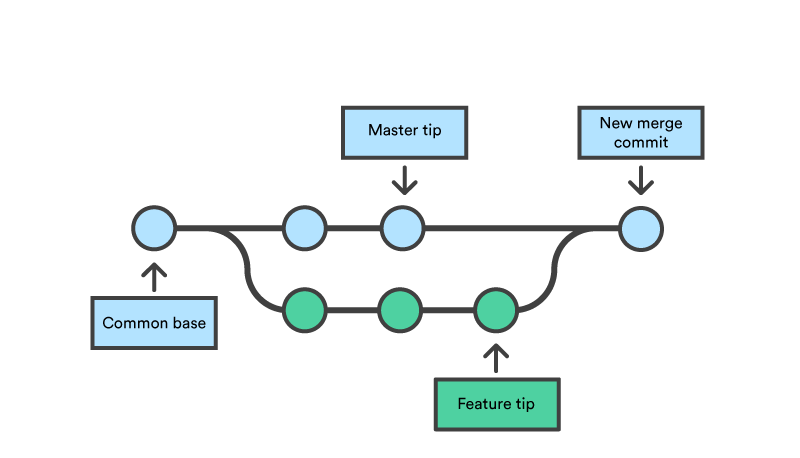
\includegraphics[width=.8\linewidth]{figs/git-branch}
\end{center}
\end{frame}


\section{Blocos}


\begin{frame}{Blocos}
	\begin{block}{Esse é um bloco}
    \begin{itemize}
        \item Isso é um teste
        \item Isso é um outro teste
    \end{itemize}
	\end{block}

	\begin{block}{}
	    Esse slide tem animação gerada pelo comando \texttt{pause}
	\end{block}

    \pause

	\begin{alertblock}{Alerta}
        Esse é um alerta
	\end{alertblock}

	\begin{exampleblock}{Bloco para exemplo}
        Exemplo com \textcolor{red}{cor em vermelho}.
    \end{exampleblock}

\end{frame}


\begin{frame}{Blocos personalizados}
    \begin{atencao}
        Isso é uma mensagem de atenção
    \end{atencao}
    \begin{informacao}
        Isso é uma mensagem de informação
    \end{informacao}
    \begin{cuidado}
        Isso é uma mensagem de cuidado
    \end{cuidado}
    
    \end{frame}


\end{document}